%%%%%%%%%%%%%%%%%%%%%%%%%%%%%%%%%%%%%%%%%%%%%%%%%%%%%%%%%%%%%%%%%%% 
%                                                                 %
%                            CHAPTER                              %
%                                                                 %
%%%%%%%%%%%%%%%%%%%%%%%%%%%%%%%%%%%%%%%%%%%%%%%%%%%%%%%%%%%%%%%%%%% 

\chapter{Bioinformatics and embedded systems}

\section{Introduction to bioinformatics}

\subsection{Biology and DNA}

\subsubsection{History of genetics and DNA}

\paragraph{Genetics}

\begin{wrapfigure}{R}{0.25\textwidth}
	%src: https://upload.wikimedia.org/wikipedia/commons/8/87/Gregor_Mendel_portrait.jpg
	\begin{center}
		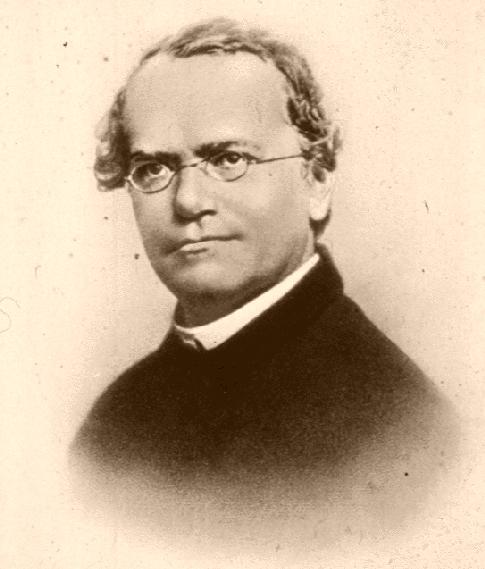
\includegraphics[width=0.20\textwidth]{background/GregorMendel.jpg}
		Gregor Mendel
	\end{center}
\end{wrapfigure}


For thousands of years, humans have observed the effects of heredity and implemented their knowledge to domesticate plants and animals. However, the science behind heredity was only started to be understood since 1859 with the publication of \emph{on the origin of species} by Charles Darwin. 

Around 1865, Austrian monk and botanist Gregor Mendel, who studied at the university in Brno in the current Czech Republic, published his results on the hybridization studies of pea plants. He is often credited as being the father of modern genetics. In his findings, he implemented the role of \emph{factors} that influence the expression of traits. These factors later became known as \emph{genes}.

\paragraph{Molecular biology}

In 1869, Swiss physician Friedrich Miescher discovered a microscopic substance in the pus of discarded surgical bandages. Later, in 1909, Phoebus Levene named this substance Deoxyribonucleic Acid (DNA) since it is found in the nucleus of a cell and has acidic properties.

The full structure of DNA was discovered by Francis Crick and James Watson at the Cavendish Laboratory at the University of Cambridge.

\subsubsection{Structure of DNA}

DNA, or Deoxyribonucleic Acid, is what stores the genetic information of all living organisms. It is the information that programs all of the activities in a cell.

Structurally, DNA is a polymer, which means each molecule is built up out of small repeating molecular units. In DNA, these units are called \emph{nucleotides}.

\begin{figure}[!ht]
	\centering
	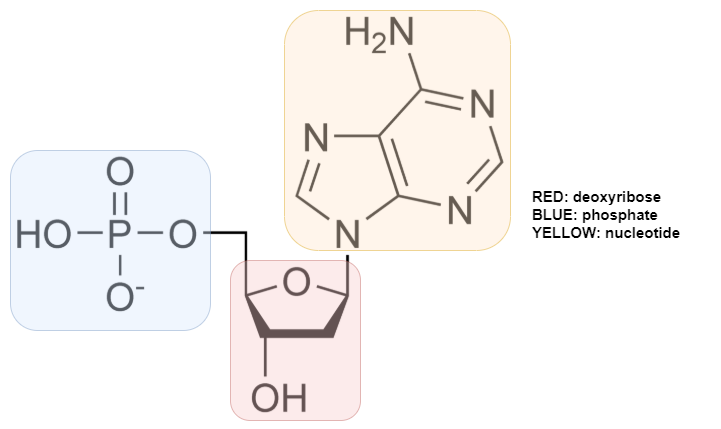
\includegraphics[width=0.75\linewidth]{background/Nucleotide.png}
	\caption{The structure of one nucleotide}
	\label{fig:nucleotide}
\end{figure}

Each nucleotide consists of 3 parts:

\begin{enumerate}
	\item A carbon sugar molecule called \emph{Deoxyribose}.
	\item A phosphate group to connect the Deoxyribose molecules with eachother. 
	\item One of four possible nitrogen bases: Adenine ($A$), Thymine ($T$), Cytosine ($C$) or Guanine ($G$).
\end{enumerate}

It is important to note that in most living organisms DNA does not exist as a single polymer, but rather a pair of molecules that are held tightly together. This is the famous \emph{double helix}.

\begin{figure}[!ht]
	%src: https://upload.wikimedia.org/wikipedia/commons/thumb/1/14/Double_stranded_DNA_with_coloured_bases.png/1024px-Double_stranded_DNA_with_coloured_bases.png
	\centering
	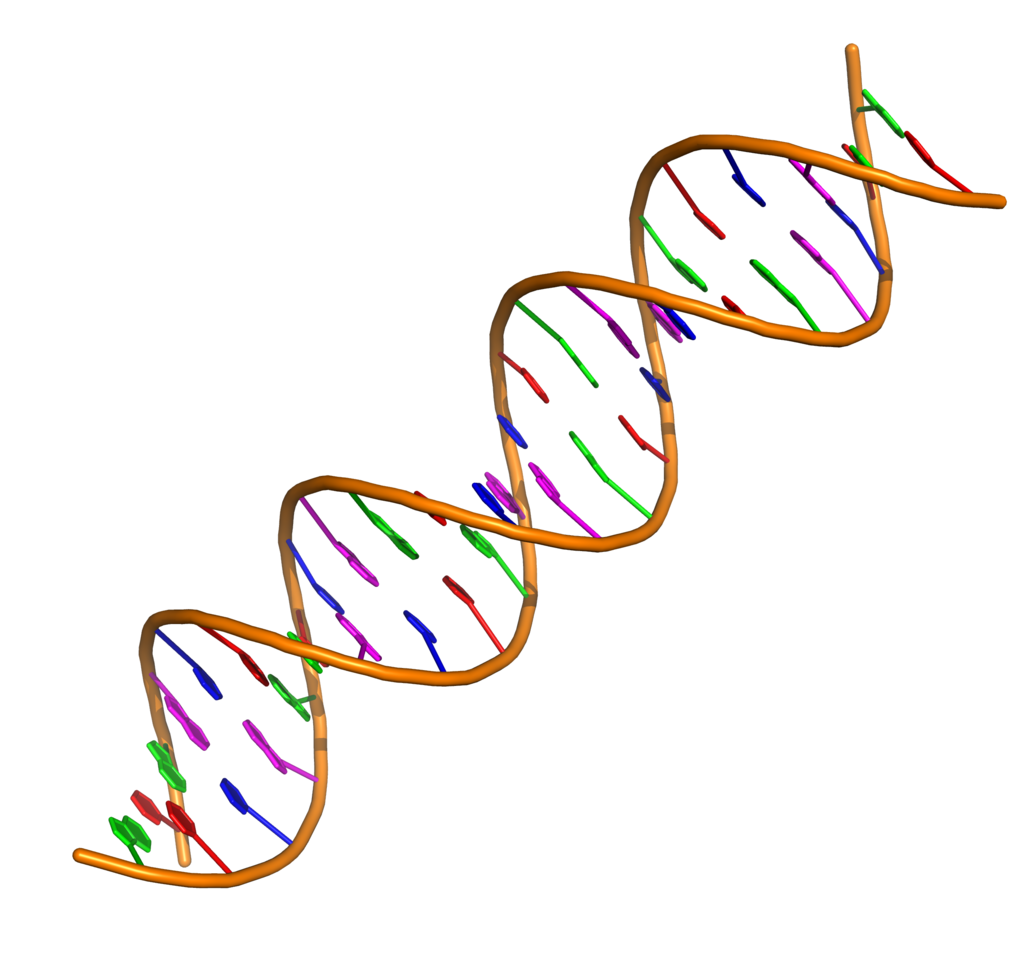
\includegraphics[width=0.3\linewidth]{background/DoubleHelix.png}
	\caption{The famous double helix}
	\label{fig:doubleHelix}
\end{figure}

Like in any good structure, there is a need for the main support. In DNA, the sugars and phosphates bond together to form twin backbones. These sugar-phosphate bonds run down each side of the helix, but chemically in opposite directions. 

The first phosphate group, at the start of the molecule, connects to the sugar group's 5th carbon. At the end of the structure, the 3rd carbon of the sugar group is unconnected. This makes a pattern typically noted as $[5' \rightarrow 3']$. Now, since the other molecule in the helix goes in the opposite direction, the pattern of the other backbone is typically noted as $[3' \rightarrow 5']$.

\begin{figure}[!ht]
	%src: https://upload.wikimedia.org/wikipedia/commons/thumb/e/e4/DNA_chemical_structure.svg/800px-DNA_chemical_structure.svg.png
	\centering
	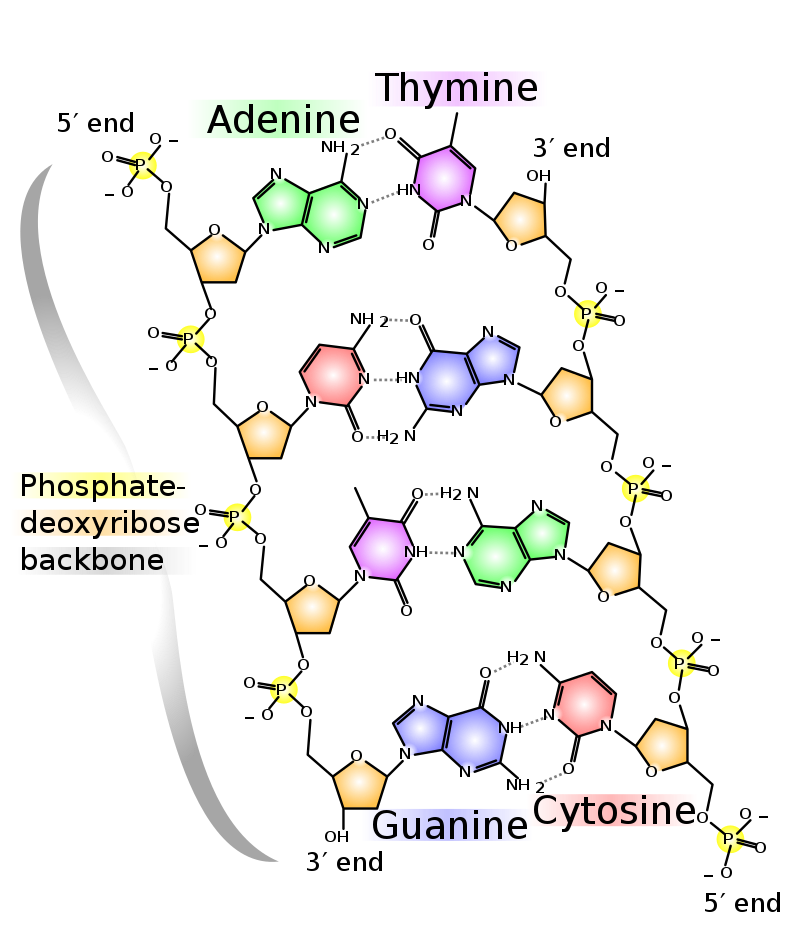
\includegraphics[width=0.5\linewidth]{background/DNAstructure.png}
	\caption{the DNA structure}
	\label{fig:DNAstructure}
\end{figure}

These two long chains are linked together by the nitrogen bases via their relatively weak hydrogen bonds, but there can't just be any pair of nitrogen bases. Adenine can only make hydrogen bonds with Thymine. Likewise, Guanine can only bond with Cytosine. These bonded nitrogen bases are called \emph{base paires}.

It is the order of these bases, which is also called the \emph{sequence}, that allows this DNA to store useful information. In this way, e.g. $AGGTCCATG$ means something completely different as a base sequence than e.g. $TTCCAGATC$.

Since each of the bases in the sequence has only one possible counterpart, you can predict what its matching counterpart will be in the opposite string. For example:

If the following sequence is known
$$[5' - AGGTCCG - 3']$$
we can deduce the sequence in the other direction as
$$[3' - TCCAGGC - 5']$$

\subsubsection{DNA in the human body}

In human cells, DNA molecules can be found in the nucleus of all cells in the body. It consists of 46 very long molecules, which during cell division condense in what we call \emph{chromosomes}. The only exception is in reproductive cells, which only have 23 chromosomes. These chromosomes are packed tightly together in the nucleus of the cell. If all of these chromosomes are put together, this makes about 3 billion base pairs. These 3 billion base pairs provide the assembly instructions for pretty much everything inside the cell.

These 46 chromosomes, which make up our whole DNA, are always present in pairs in the cells. Each time, the pair consists of one chromosome from each parent. 

These 23 chromosome pairs are classified in 
\begin{itemize}
	\item 22 pairs of autosomal chromosomes. These are marked 1 to 22 according to the length of the sequence. The longest chromosome (chromosome number-1) is 248,956,422 bases long. The shortest (chromosome number-22) is 50,818,468 bases long.
	\item In each cell, there is also an X chromosome plus an X or Y, dependent on the gender.
\end{itemize}


\begin{figure}[!ht]
	%src: https://upload.wikimedia.org/wikipedia/commons/thumb/b/b2/Karyotype.png/800px-Karyotype.png
	\centering
	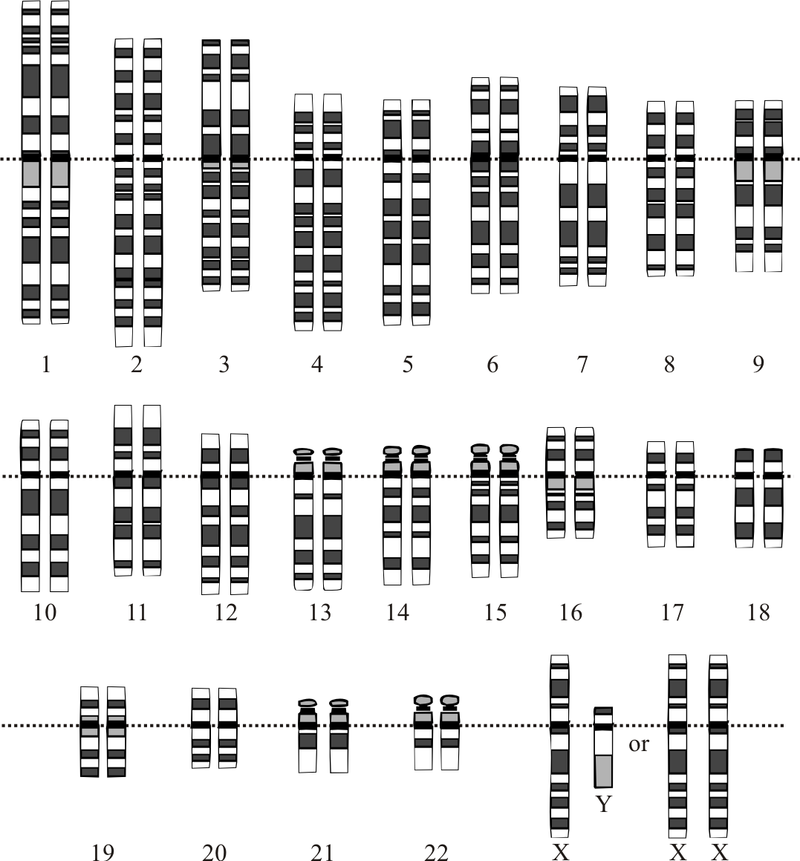
\includegraphics[width=0.5\linewidth]{background/karyotype.png}
	\caption{the human chromosomes}
	\label{fig:karyotype}
\end{figure}


\subsection{Sequencing and the need for Bioinformatics}



\subsection{DNA sequence aligning}



\subsection{Clinical applications}




\section{Platforms for sequence alignment algorithms}

\subsection{CPU}
\subsection{GPU}
\subsection{FPGA}
\subsection{ASIC}

\section{Problem definition}